%!TEX root=../oi-magistr-spolecne.tex
\section[KO - SPT, TSP, knapsack]{Nejkratší cesty. Úloha obchodního cestujícího. Heuristiky a aproximační algoritmy. Metoda dynamického programování. Problém batohu. Pseudo-polynomiální algoritmy.}

\begin{enumerate}
\item SPT - definovat, spousta problemu se na to da prevezt, trojuhelnikova nerovnost\item TSP - definovat, slozitost, dukaz NP z redukce z Ham Cycle + dukaz neexistence aprox alg, heuristiky 2 aprox atd\item Knapsack - definovat, dynamicke programovani, 2aprox, pseudo polym alg
\end{enumerate}

Nejkratší cesta je problém nalezení nejkratší cesty z x do y. V obecném grafu se zápornými cykly je to NP-úplná úloha.

Bellmanova rovnice: Pokud graf neobsahuje záporné cykly, nejkratší cesta x,y se skládá s cesty x, z + z,y, tak aby byl součet minimální. Tzn. nejkratší cesta se skládá s dílčích nejkratších cest.

Dijkstra: Funguje pokud nejsou záporné hrany. Algoritmus má uzly v prioritní frontě podle vzdálenosti od zdroje. Na začátku zdroj 0, ostatní nekonečno. Vždy odebere uzel s nejmenší vzdáleností a provede tzv. relaxaci - podívá se na všechny sousedy ještě ve frontě a ověří, jestli se tam přes tento uzel nejde dostat rychleji. Pokud ano, sníží prioritu. Když odebereme cílový uzel, algoritmus končí. Je dobré si zaznamenávat předchůdce. $O(E\cdot \log V)$.

Bellman-Ford: podobný Dijkstrovi, ale funguje pro hrany záporné délky. Může také detekovat záporný cyklus. Probíhá tak, že pro každý uzel se provede relaxace. $O(E\cdot V)$

Floyd-Warshall: najde nejkratší cesty od všech uzlů ke všem, detekuje záporné cykly. Nejdřív matice kdo s kým sousedí, iteruju k=1..n. Procházím všechny prvky a dívám se co protínám v k-tém řádku a sloupci. Sečtu ty prvky. Když je součet menší, nahradím. Při náhradách je dobré vést matici předchůdců. Když bude <0 na diagonále, záporný cyklus. $O(E^2 \cdot V)$.

\subsection{Úloha obchodního cestujícího (TSP)}
TSP je nalezení nejkratší hamiltonovské kružnice v ohodnoceném grafu. Je silně NP-obtížná = neexistuje k-aproximační algoritmus. V metrickém TSP (vzdálenosti splňují trojúhelníkovou nerovnost) ale jde aproximovat: 2-aproximační algoritmus: Nalezne se kostra Kruskalem a vypíše se první výskyt uzlů při procházení do hloubky 3/2-aproximační algoritmus (Christofidesův): obtížnější implementace, na reálných datech není v průměrném případě o moc lepší. Důkaz NP-hard: Mějme graf G, kde rozhodujeme jestli tam je hamilton. kružnice. Vytvoříme instanci TSP - úplný graf, kde ceny budou 1 pokud ta hrana byla v grafu G a 2 pokud nebyla v grafu G. G má hamiltonovskou kružnici když řešení TSP = n => TSP je silně NP-hard.

Heuristika je postup jak rychle získat sub-optimální řešení problému, které může být good enough. Např. pokus a omyl, genetický algoritmus, hladový algoritmus - při prohledávání si podle heuristiky vybereme kam jít.

Aproximační algoritmy - je u nich dokázáno, že nikdy nebudou horší než k. Třeba 2-aproximační algoritmus pro TSP.

\subsection{Batoh (Knapsack)}
Problém batohu (Knapsack) řeší problém, které předměty dát do batohu tak, aby nebyla překročena kapacita a celková cena byla maximální. Hladový algoritmus funguje pokud máme neomezeně předmětů. Prostě seřadíme předměty podle poměru cena/váha a dáváme je do batohu. Pak je 2-aproximační. Dynamické programování může vyřešit pseudo-polynomiálně. Mám tabulku číslo rozhodnutí x váha. Vždy se větvím na dva - přidám nebo nepřidám. Posunu se dolů o 1 a vpravo kolik tím přibyde váhy. Když překročím kapacitu, ořez. Do políček zapisuju celkovou cenu. Když už na políčku něco je, nahrazuji jenom menší cenu. Nejvíc vpravo dole bude optimální řešení.

\begin{figure}[h]
    \begin{center}
        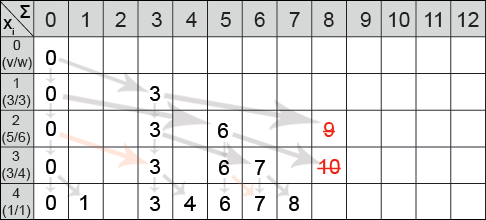
\includegraphics[width=100mm]{09/images/knapsack}
    \end{center}
    \caption{Batoh o kapacitě 8 a předměty s váhami: $[3,6,4,1]$, hodnotami $[3, 5, 3, 1]$}
\end{figure}

Pseudo-polynomiální algoritmy mají složitost O(C n), kde C nezáleží na velikosti instance (n) a může být hodně velké, až exponenciální. Např. algoritmus dynamického programování pro Knapsack.
